\documentclass[twoside]{book}

% Packages required by doxygen
\usepackage{fixltx2e}
\usepackage{calc}
\usepackage{doxygen}
\usepackage[export]{adjustbox} % also loads graphicx
\usepackage{graphicx}
\usepackage[utf8]{inputenc}
\usepackage{makeidx}
\usepackage{multicol}
\usepackage{multirow}
\PassOptionsToPackage{warn}{textcomp}
\usepackage{textcomp}
\usepackage[nointegrals]{wasysym}
\usepackage[table]{xcolor}

% Font selection
\usepackage[T1]{fontenc}
\usepackage[scaled=.90]{helvet}
\usepackage{courier}
\usepackage{amssymb}
\usepackage{sectsty}
\renewcommand{\familydefault}{\sfdefault}
\allsectionsfont{%
  \fontseries{bc}\selectfont%
  \color{darkgray}%
}
\renewcommand{\DoxyLabelFont}{%
  \fontseries{bc}\selectfont%
  \color{darkgray}%
}
\newcommand{\+}{\discretionary{\mbox{\scriptsize$\hookleftarrow$}}{}{}}

% Page & text layout
\usepackage{geometry}
\geometry{%
  a4paper,%
  top=2.5cm,%
  bottom=2.5cm,%
  left=2.5cm,%
  right=2.5cm%
}
\tolerance=750
\hfuzz=15pt
\hbadness=750
\setlength{\emergencystretch}{15pt}
\setlength{\parindent}{0cm}
\setlength{\parskip}{0.2cm}
\makeatletter
\renewcommand{\paragraph}{%
  \@startsection{paragraph}{4}{0ex}{-1.0ex}{1.0ex}{%
    \normalfont\normalsize\bfseries\SS@parafont%
  }%
}
\renewcommand{\subparagraph}{%
  \@startsection{subparagraph}{5}{0ex}{-1.0ex}{1.0ex}{%
    \normalfont\normalsize\bfseries\SS@subparafont%
  }%
}
\makeatother

% Headers & footers
\usepackage{fancyhdr}
\pagestyle{fancyplain}
\fancyhead[LE]{\fancyplain{}{\bfseries\thepage}}
\fancyhead[CE]{\fancyplain{}{}}
\fancyhead[RE]{\fancyplain{}{\bfseries\leftmark}}
\fancyhead[LO]{\fancyplain{}{\bfseries\rightmark}}
\fancyhead[CO]{\fancyplain{}{}}
\fancyhead[RO]{\fancyplain{}{\bfseries\thepage}}
\fancyfoot[LE]{\fancyplain{}{}}
\fancyfoot[CE]{\fancyplain{}{}}
\fancyfoot[RE]{\fancyplain{}{\bfseries\scriptsize Generated on Tue Nov 24 2015 07\+:04\+:39 for S\+P\+H by Doxygen }}
\fancyfoot[LO]{\fancyplain{}{\bfseries\scriptsize Generated on Tue Nov 24 2015 07\+:04\+:39 for S\+P\+H by Doxygen }}
\fancyfoot[CO]{\fancyplain{}{}}
\fancyfoot[RO]{\fancyplain{}{}}
\renewcommand{\footrulewidth}{0.4pt}
\renewcommand{\chaptermark}[1]{%
  \markboth{#1}{}%
}
\renewcommand{\sectionmark}[1]{%
  \markright{\thesection\ #1}%
}

% Indices & bibliography
\usepackage{natbib}
\usepackage[titles]{tocloft}
\setcounter{tocdepth}{3}
\setcounter{secnumdepth}{5}
\makeindex

% Hyperlinks (required, but should be loaded last)
\usepackage{ifpdf}
\ifpdf
  \usepackage[pdftex,pagebackref=true]{hyperref}
\else
  \usepackage[ps2pdf,pagebackref=true]{hyperref}
\fi
\hypersetup{%
  colorlinks=true,%
  linkcolor=blue,%
  citecolor=blue,%
  unicode%
}

% Custom commands
\newcommand{\clearemptydoublepage}{%
  \newpage{\pagestyle{empty}\cleardoublepage}%
}


%===== C O N T E N T S =====

\begin{document}

% Titlepage & ToC
\hypersetup{pageanchor=false,
             bookmarks=true,
             bookmarksnumbered=true,
             pdfencoding=unicode
            }
\pagenumbering{roman}
\begin{titlepage}
\vspace*{7cm}
\begin{center}%
{\Large S\+P\+H }\\
\vspace*{1cm}
{\large Generated by Doxygen 1.8.9.1}\\
\vspace*{0.5cm}
{\small Tue Nov 24 2015 07:04:39}\\
\end{center}
\end{titlepage}
\clearemptydoublepage
\tableofcontents
\clearemptydoublepage
\pagenumbering{arabic}
\hypersetup{pageanchor=true}

%--- Begin generated contents ---
\chapter{Class Index}
\section{Class List}
Here are the classes, structs, unions and interfaces with brief descriptions\+:\begin{DoxyCompactList}
\item\contentsline{section}{\hyperlink{classAABB}{A\+A\+B\+B$<$ Real, dim $>$} }{\pageref{classAABB}}{}
\item\contentsline{section}{\hyperlink{classAABB_3_01Real_00_01three__dimensional_01_4}{A\+A\+B\+B$<$ Real, three\+\_\+dimensional $>$} }{\pageref{classAABB_3_01Real_00_01three__dimensional_01_4}}{}
\item\contentsline{section}{\hyperlink{classAABB_3_01Real_00_01two__dimensional_01_4}{A\+A\+B\+B$<$ Real, two\+\_\+dimensional $>$} }{\pageref{classAABB_3_01Real_00_01two__dimensional_01_4}}{}
\item\contentsline{section}{\hyperlink{classAdiosWriter}{Adios\+Writer$<$ Real, Dim $>$} }{\pageref{classAdiosWriter}}{}
\item\contentsline{section}{\hyperlink{classDistributor}{Distributor$<$ Real, Dim $>$} }{\pageref{classDistributor}}{}
\item\contentsline{section}{\hyperlink{classKernels}{Kernels$<$ Real, Dim $>$} }{\pageref{classKernels}}{}
\item\contentsline{section}{\hyperlink{classNeighbors}{Neighbors$<$ Real, Dim $>$} }{\pageref{classNeighbors}}{}
\item\contentsline{section}{\hyperlink{classParameters}{Parameters$<$ Real, Dim $>$} }{\pageref{classParameters}}{}
\item\contentsline{section}{\hyperlink{classParticles}{Particles$<$ Real, Dim $>$} }{\pageref{classParticles}}{}
\item\contentsline{section}{\hyperlink{classSimulation}{Simulation$<$ Real, Dim $>$} }{\pageref{classSimulation}}{}
\item\contentsline{section}{\hyperlink{structVec}{Vec$<$ T, n $>$} \\*Generic n-\/dim \hyperlink{structVec}{Vec} implementation }{\pageref{structVec}}{}
\item\contentsline{section}{\hyperlink{structVec_3_01T_00_012_01_4}{Vec$<$ T, 2 $>$} }{\pageref{structVec_3_01T_00_012_01_4}}{}
\item\contentsline{section}{\hyperlink{structVec_3_01T_00_013_01_4}{Vec$<$ T, 3 $>$} }{\pageref{structVec_3_01T_00_013_01_4}}{}
\end{DoxyCompactList}

\chapter{Class Documentation}
\hypertarget{classAABB}{}\section{A\+A\+B\+B$<$ Real, dim $>$ Class Template Reference}
\label{classAABB}\index{A\+A\+B\+B$<$ Real, dim $>$@{A\+A\+B\+B$<$ Real, dim $>$}}


{\ttfamily \#include $<$aabb.\+h$>$}



\subsection{Detailed Description}
\subsubsection*{template$<$typename Real, Dimension dim$>$class A\+A\+B\+B$<$ Real, dim $>$}

Class to handle Axis aligned boundary box and 2\+D equivalent 

The documentation for this class was generated from the following file\+:\begin{DoxyCompactItemize}
\item 
/home/atj/\+Dropbox/\+S\+P\+H\+P\+C/\+Simulation\+\_\+\+C\+C/src/aabb.\+h\end{DoxyCompactItemize}

\hypertarget{classAABB_3_01Real_00_01three__dimensional_01_4}{}\section{A\+A\+B\+B$<$ Real, three\+\_\+dimensional $>$ Class Template Reference}
\label{classAABB_3_01Real_00_01three__dimensional_01_4}\index{A\+A\+B\+B$<$ Real, three\+\_\+dimensional $>$@{A\+A\+B\+B$<$ Real, three\+\_\+dimensional $>$}}


Collaboration diagram for A\+A\+B\+B$<$ Real, three\+\_\+dimensional $>$\+:\nopagebreak
\begin{figure}[H]
\begin{center}
\leavevmode
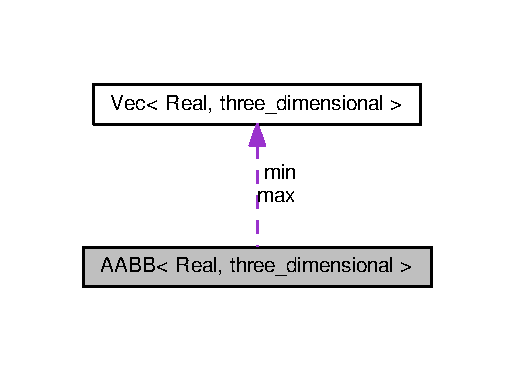
\includegraphics[width=247pt]{classAABB_3_01Real_00_01three__dimensional_01_4__coll__graph}
\end{center}
\end{figure}
\subsection*{Public Member Functions}
\begin{DoxyCompactItemize}
\item 
\hypertarget{classAABB_3_01Real_00_01three__dimensional_01_4_aba455f7183e007051b93e405fe474621}{}Real {\bfseries Length} () const \label{classAABB_3_01Real_00_01three__dimensional_01_4_aba455f7183e007051b93e405fe474621}

\item 
\hypertarget{classAABB_3_01Real_00_01three__dimensional_01_4_ad3456e9fb2e64df7567b8cdedcd2c614}{}Real {\bfseries Height} () const \label{classAABB_3_01Real_00_01three__dimensional_01_4_ad3456e9fb2e64df7567b8cdedcd2c614}

\item 
\hypertarget{classAABB_3_01Real_00_01three__dimensional_01_4_a719fc794b4792918aefd2e1ee4014dc6}{}Real {\bfseries Depth} () const \label{classAABB_3_01Real_00_01three__dimensional_01_4_a719fc794b4792918aefd2e1ee4014dc6}

\item 
\hypertarget{classAABB_3_01Real_00_01three__dimensional_01_4_adadc6a1e70c803de43969200d5012d49}{}Real {\bfseries Volume} () const \label{classAABB_3_01Real_00_01three__dimensional_01_4_adadc6a1e70c803de43969200d5012d49}

\end{DoxyCompactItemize}
\subsection*{Public Attributes}
\begin{DoxyCompactItemize}
\item 
\hypertarget{classAABB_3_01Real_00_01three__dimensional_01_4_a94bd63d979c7cdb4ebc061131309dd37}{}\hyperlink{structVec}{Vec}$<$ Real, three\+\_\+dimensional $>$ {\bfseries min}\label{classAABB_3_01Real_00_01three__dimensional_01_4_a94bd63d979c7cdb4ebc061131309dd37}

\item 
\hypertarget{classAABB_3_01Real_00_01three__dimensional_01_4_a6aafd1c321e46a76831a702af4ea9157}{}\hyperlink{structVec}{Vec}$<$ Real, three\+\_\+dimensional $>$ {\bfseries max}\label{classAABB_3_01Real_00_01three__dimensional_01_4_a6aafd1c321e46a76831a702af4ea9157}

\end{DoxyCompactItemize}


The documentation for this class was generated from the following file\+:\begin{DoxyCompactItemize}
\item 
/home/atj/\+Dropbox/\+S\+P\+H\+P\+C/\+Simulation\+\_\+\+C\+C/src/aabb.\+h\end{DoxyCompactItemize}

\hypertarget{classAABB_3_01Real_00_01two__dimensional_01_4}{}\section{A\+A\+B\+B$<$ Real, two\+\_\+dimensional $>$ Class Template Reference}
\label{classAABB_3_01Real_00_01two__dimensional_01_4}\index{A\+A\+B\+B$<$ Real, two\+\_\+dimensional $>$@{A\+A\+B\+B$<$ Real, two\+\_\+dimensional $>$}}


Collaboration diagram for A\+A\+B\+B$<$ Real, two\+\_\+dimensional $>$\+:\nopagebreak
\begin{figure}[H]
\begin{center}
\leavevmode
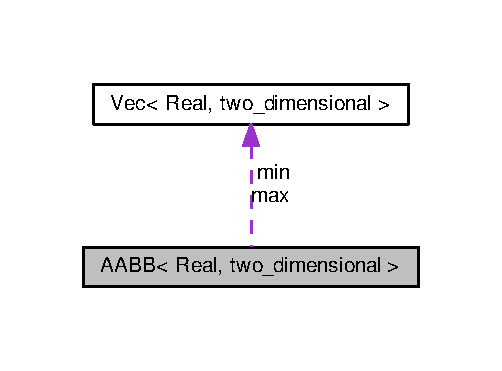
\includegraphics[width=241pt]{classAABB_3_01Real_00_01two__dimensional_01_4__coll__graph}
\end{center}
\end{figure}
\subsection*{Public Member Functions}
\begin{DoxyCompactItemize}
\item 
\hypertarget{classAABB_3_01Real_00_01two__dimensional_01_4_a65a6648938ef13ecf6cd5fcbe14870db}{}Real {\bfseries Length} () const \label{classAABB_3_01Real_00_01two__dimensional_01_4_a65a6648938ef13ecf6cd5fcbe14870db}

\item 
\hypertarget{classAABB_3_01Real_00_01two__dimensional_01_4_a4a6aeef68085a0add92352726069a99d}{}Real {\bfseries Height} () const \label{classAABB_3_01Real_00_01two__dimensional_01_4_a4a6aeef68085a0add92352726069a99d}

\item 
\hypertarget{classAABB_3_01Real_00_01two__dimensional_01_4_abeeebf41b3ac413f825148fe28a03669}{}Real {\bfseries Volume} () const \label{classAABB_3_01Real_00_01two__dimensional_01_4_abeeebf41b3ac413f825148fe28a03669}

\end{DoxyCompactItemize}
\subsection*{Public Attributes}
\begin{DoxyCompactItemize}
\item 
\hypertarget{classAABB_3_01Real_00_01two__dimensional_01_4_a270e28f2f508e7489c3e46905621c4df}{}\hyperlink{structVec}{Vec}$<$ Real, two\+\_\+dimensional $>$ {\bfseries min}\label{classAABB_3_01Real_00_01two__dimensional_01_4_a270e28f2f508e7489c3e46905621c4df}

\item 
\hypertarget{classAABB_3_01Real_00_01two__dimensional_01_4_ad5b370374a2357bd82b596e4d09fea2d}{}\hyperlink{structVec}{Vec}$<$ Real, two\+\_\+dimensional $>$ {\bfseries max}\label{classAABB_3_01Real_00_01two__dimensional_01_4_ad5b370374a2357bd82b596e4d09fea2d}

\end{DoxyCompactItemize}


The documentation for this class was generated from the following file\+:\begin{DoxyCompactItemize}
\item 
/home/atj/\+Dropbox/\+S\+P\+H\+P\+C/\+Simulation\+\_\+\+C\+C/src/aabb.\+h\end{DoxyCompactItemize}

\hypertarget{classAdiosWriter}{}\section{Adios\+Writer$<$ Real, Dim $>$ Class Template Reference}
\label{classAdiosWriter}\index{Adios\+Writer$<$ Real, Dim $>$@{Adios\+Writer$<$ Real, Dim $>$}}
\subsection*{Public Member Functions}
\begin{DoxyCompactItemize}
\item 
\hypertarget{classAdiosWriter_a51608b20d79e69dca7e1a8e9f6899cb4}{}{\bfseries Adios\+Writer} (const std\+::string \&adios\+\_\+writer\+\_\+xml, const \hyperlink{classDistributor}{Distributor}$<$ Real, Dim $>$ \&distributor\+\_\+, const \hyperlink{classParticles}{Particles}$<$ Real, Dim $>$ \&particles\+\_\+, const \hyperlink{classParameters}{Parameters}$<$ Real, Dim $>$ \&parameters\+\_\+)\label{classAdiosWriter_a51608b20d79e69dca7e1a8e9f6899cb4}

\item 
\hypertarget{classAdiosWriter_a0e7286883597308c953d3822c78b2aab}{}{\bfseries Adios\+Writer} (const \hyperlink{classAdiosWriter}{Adios\+Writer} \&)=delete\label{classAdiosWriter_a0e7286883597308c953d3822c78b2aab}

\item 
\hypertarget{classAdiosWriter_af3d244b8ec6c45ca140dae5f992eb9ba}{}\hyperlink{classAdiosWriter}{Adios\+Writer} \& {\bfseries operator=} (const \hyperlink{classAdiosWriter}{Adios\+Writer} \&)=delete\label{classAdiosWriter_af3d244b8ec6c45ca140dae5f992eb9ba}

\item 
\hypertarget{classAdiosWriter_a5fb32706200c08a7c2f4f2e6aa1768aa}{}{\bfseries Adios\+Writer} (\hyperlink{classAdiosWriter}{Adios\+Writer} \&\&) noexcept=delete\label{classAdiosWriter_a5fb32706200c08a7c2f4f2e6aa1768aa}

\item 
\hypertarget{classAdiosWriter_a54a40b63a55d6aaef0dbcb074f4bcba0}{}\hyperlink{classAdiosWriter}{Adios\+Writer} \& {\bfseries operator=} (\hyperlink{classAdiosWriter}{Adios\+Writer} \&\&)=delete\label{classAdiosWriter_a54a40b63a55d6aaef0dbcb074f4bcba0}

\item 
void \hyperlink{classAdiosWriter_ac26ceaab9a7ecda73c2cd4d2d9117afa}{Write\+Particles} ()
\end{DoxyCompactItemize}


\subsection{Member Function Documentation}
\hypertarget{classAdiosWriter_ac26ceaab9a7ecda73c2cd4d2d9117afa}{}\index{Adios\+Writer@{Adios\+Writer}!Write\+Particles@{Write\+Particles}}
\index{Write\+Particles@{Write\+Particles}!Adios\+Writer@{Adios\+Writer}}
\subsubsection[{Write\+Particles}]{\setlength{\rightskip}{0pt plus 5cm}template$<$typename Real, Dimension Dim$>$ void {\bf Adios\+Writer}$<$ Real, Dim $>$\+::Write\+Particles (
\begin{DoxyParamCaption}
{}
\end{DoxyParamCaption}
)\hspace{0.3cm}{\ttfamily [inline]}}\label{classAdiosWriter_ac26ceaab9a7ecda73c2cd4d2d9117afa}
Write particle coordinates 

The documentation for this class was generated from the following file\+:\begin{DoxyCompactItemize}
\item 
/home/atj/\+Dropbox/\+S\+P\+H\+P\+C/\+Simulation\+\_\+\+C\+C/src/adios\+\_\+writer.\+h\end{DoxyCompactItemize}

\hypertarget{classDistributor}{}\section{Distributor$<$ Real, Dim $>$ Class Template Reference}
\label{classDistributor}\index{Distributor$<$ Real, Dim $>$@{Distributor$<$ Real, Dim $>$}}
\subsection*{Public Member Functions}
\begin{DoxyCompactItemize}
\item 
\hyperlink{classDistributor_a28b0eb640ee22135e0566d2fc29abfb4}{Distributor} (const \hyperlink{classParameters}{Parameters}$<$ Real, Dim $>$ \&params, \hyperlink{classParticles}{Particles}$<$ Real, Dim $>$ \&particles\+\_\+)
\item 
\hypertarget{classDistributor_a73ef5ca71d4cff8fffd87f3b42922fad}{}{\bfseries Distributor} (const \hyperlink{classDistributor}{Distributor} \&)=delete\label{classDistributor_a73ef5ca71d4cff8fffd87f3b42922fad}

\item 
\hypertarget{classDistributor_abcc51f27dfc345acf264642c338fa7e3}{}\hyperlink{classDistributor}{Distributor} \& {\bfseries operator=} (const \hyperlink{classDistributor}{Distributor} \&)=delete\label{classDistributor_abcc51f27dfc345acf264642c338fa7e3}

\item 
\hypertarget{classDistributor_a7c5ecf5f7f912c758317b8cfd85f7f76}{}{\bfseries Distributor} (\hyperlink{classDistributor}{Distributor} \&\&) noexcept=delete\label{classDistributor_a7c5ecf5f7f912c758317b8cfd85f7f76}

\item 
\hypertarget{classDistributor_a6b02405b5ed14d90a4baf3441521cab0}{}\hyperlink{classDistributor}{Distributor} \& {\bfseries operator=} (\hyperlink{classDistributor}{Distributor} \&\&)=delete\label{classDistributor_a6b02405b5ed14d90a4baf3441521cab0}

\item 
void \hyperlink{classDistributor_a1468124b3b60be412af5d0c1c4b9384f}{Initilize} ()
\item 
void \hyperlink{classDistributor_a0a57fa982d214c7f02f40875bde3d866}{Set\+Node\+Bounds} (const \hyperlink{classAABB}{A\+A\+B\+B}$<$ Real, Dim $>$ \&aabb)
\item 
\hypertarget{classDistributor_a0b4db4298e86c87f62f2301905666af8}{}bool {\bfseries Last\+Node} () const \label{classDistributor_a0b4db4298e86c87f62f2301905666af8}

\item 
int \hyperlink{classDistributor_a6d353a3fa6453bd0db5c5d188ae2b2cf}{Node\+To\+Left} () const 
\item 
int \hyperlink{classDistributor_ae1a47636aa4afc7f3b131fb5fb526a3b}{Node\+To\+Right} () const 
\item 
\hypertarget{classDistributor_a674dc3cd0d8cd86b7d1a16e91578af92}{}boost\+::mpi\+::communicator {\bfseries Get\+Active\+Comm} () const \label{classDistributor_a674dc3cd0d8cd86b7d1a16e91578af92}

\item 
\hypertarget{classDistributor_aa95007c8f91e2f3bd4bbb59f6d7b117f}{}int {\bfseries Get\+Active\+Rank} () const \label{classDistributor_aa95007c8f91e2f3bd4bbb59f6d7b117f}

\item 
void \hyperlink{classDistributor_a79ed97a84dac0188440b12c6dc73c938}{Distribute\+Fluid} (const \hyperlink{classAABB}{A\+A\+B\+B}$<$ Real, Dim $>$ \&global\+\_\+fluid)
\item 
\hypertarget{classDistributor_a3ca5328dd7a2bafd3d0b18db85bd7d4d}{}std\+::size\+\_\+t {\bfseries Get\+Global\+Particle\+Count} () const \label{classDistributor_a3ca5328dd7a2bafd3d0b18db85bd7d4d}

\end{DoxyCompactItemize}


\subsection{Constructor \& Destructor Documentation}
\hypertarget{classDistributor_a28b0eb640ee22135e0566d2fc29abfb4}{}\index{Distributor@{Distributor}!Distributor@{Distributor}}
\index{Distributor@{Distributor}!Distributor@{Distributor}}
\subsubsection[{Distributor}]{\setlength{\rightskip}{0pt plus 5cm}template$<$typename Real, Dimension Dim$>$ {\bf Distributor}$<$ Real, Dim $>$\+::{\bf Distributor} (
\begin{DoxyParamCaption}
\item[{const {\bf Parameters}$<$ Real, Dim $>$ \&}]{params, }
\item[{{\bf Particles}$<$ Real, Dim $>$ \&}]{particles\+\_\+}
\end{DoxyParamCaption}
)\hspace{0.3cm}{\ttfamily [inline]}}\label{classDistributor_a28b0eb640ee22135e0566d2fc29abfb4}
\hyperlink{classDistributor}{Distributor} Constructor\+: Don\textquotesingle{}t use member references! \hyperlink{classDistributor}{Distributor} must be constructed before any other members 

\subsection{Member Function Documentation}
\hypertarget{classDistributor_a79ed97a84dac0188440b12c6dc73c938}{}\index{Distributor@{Distributor}!Distribute\+Fluid@{Distribute\+Fluid}}
\index{Distribute\+Fluid@{Distribute\+Fluid}!Distributor@{Distributor}}
\subsubsection[{Distribute\+Fluid}]{\setlength{\rightskip}{0pt plus 5cm}template$<$typename Real, Dimension Dim$>$ void {\bf Distributor}$<$ Real, Dim $>$\+::Distribute\+Fluid (
\begin{DoxyParamCaption}
\item[{const {\bf A\+A\+B\+B}$<$ Real, Dim $>$ \&}]{global\+\_\+fluid}
\end{DoxyParamCaption}
)\hspace{0.3cm}{\ttfamily [inline]}}\label{classDistributor_a79ed97a84dac0188440b12c6dc73c938}
Construct water volume spread across multiple nodes \hypertarget{classDistributor_a1468124b3b60be412af5d0c1c4b9384f}{}\index{Distributor@{Distributor}!Initilize@{Initilize}}
\index{Initilize@{Initilize}!Distributor@{Distributor}}
\subsubsection[{Initilize}]{\setlength{\rightskip}{0pt plus 5cm}template$<$typename Real, Dimension Dim$>$ void {\bf Distributor}$<$ Real, Dim $>$\+::Initilize (
\begin{DoxyParamCaption}
{}
\end{DoxyParamCaption}
)\hspace{0.3cm}{\ttfamily [inline]}}\label{classDistributor_a1468124b3b60be412af5d0c1c4b9384f}
Handle setting initial node boundaries required as members not being initilized when constructor is called \hypertarget{classDistributor_a6d353a3fa6453bd0db5c5d188ae2b2cf}{}\index{Distributor@{Distributor}!Node\+To\+Left@{Node\+To\+Left}}
\index{Node\+To\+Left@{Node\+To\+Left}!Distributor@{Distributor}}
\subsubsection[{Node\+To\+Left}]{\setlength{\rightskip}{0pt plus 5cm}template$<$typename Real, Dimension Dim$>$ int {\bf Distributor}$<$ Real, Dim $>$\+::Node\+To\+Left (
\begin{DoxyParamCaption}
{}
\end{DoxyParamCaption}
) const\hspace{0.3cm}{\ttfamily [inline]}}\label{classDistributor_a6d353a3fa6453bd0db5c5d188ae2b2cf}
Return rank of node to the left or M\+P\+I\+\_\+\+P\+R\+O\+C\+\_\+\+N\+U\+L\+L \hypertarget{classDistributor_ae1a47636aa4afc7f3b131fb5fb526a3b}{}\index{Distributor@{Distributor}!Node\+To\+Right@{Node\+To\+Right}}
\index{Node\+To\+Right@{Node\+To\+Right}!Distributor@{Distributor}}
\subsubsection[{Node\+To\+Right}]{\setlength{\rightskip}{0pt plus 5cm}template$<$typename Real, Dimension Dim$>$ int {\bf Distributor}$<$ Real, Dim $>$\+::Node\+To\+Right (
\begin{DoxyParamCaption}
{}
\end{DoxyParamCaption}
) const\hspace{0.3cm}{\ttfamily [inline]}}\label{classDistributor_ae1a47636aa4afc7f3b131fb5fb526a3b}
Return rank of node to the right or M\+P\+I\+\_\+\+P\+R\+O\+C\+\_\+\+N\+U\+L\+L \hypertarget{classDistributor_a0a57fa982d214c7f02f40875bde3d866}{}\index{Distributor@{Distributor}!Set\+Node\+Bounds@{Set\+Node\+Bounds}}
\index{Set\+Node\+Bounds@{Set\+Node\+Bounds}!Distributor@{Distributor}}
\subsubsection[{Set\+Node\+Bounds}]{\setlength{\rightskip}{0pt plus 5cm}template$<$typename Real, Dimension Dim$>$ void {\bf Distributor}$<$ Real, Dim $>$\+::Set\+Node\+Bounds (
\begin{DoxyParamCaption}
\item[{const {\bf A\+A\+B\+B}$<$ Real, Dim $>$ \&}]{aabb}
\end{DoxyParamCaption}
)\hspace{0.3cm}{\ttfamily [inline]}}\label{classDistributor_a0a57fa982d214c7f02f40875bde3d866}
Set node bounds based upon equal spacing in \hyperlink{classAABB}{A\+A\+B\+B} 

The documentation for this class was generated from the following file\+:\begin{DoxyCompactItemize}
\item 
/home/atj/\+Dropbox/\+S\+P\+H\+P\+C/\+Simulation\+\_\+\+C\+C/src/distributor.\+h\end{DoxyCompactItemize}

\hypertarget{classKernels}{}\section{Kernels$<$ Real, Dim $>$ Class Template Reference}
\label{classKernels}\index{Kernels$<$ Real, Dim $>$@{Kernels$<$ Real, Dim $>$}}
\subsection*{Public Member Functions}
\begin{DoxyCompactItemize}
\item 
\hypertarget{classKernels_a624c777a16ae45da518cded92949c9c6}{}{\bfseries Kernels} (const \hyperlink{classParameters}{Parameters}$<$ Real, Dim $>$ \&params)\label{classKernels_a624c777a16ae45da518cded92949c9c6}

\item 
\hypertarget{classKernels_a6656e4a55980d231b057e42c79ae2093}{}Real {\bfseries Poly6} ()\label{classKernels_a6656e4a55980d231b057e42c79ae2093}

\end{DoxyCompactItemize}


The documentation for this class was generated from the following file\+:\begin{DoxyCompactItemize}
\item 
/home/atj/\+Dropbox/\+S\+P\+H\+P\+C/\+Simulation\+\_\+\+C\+C/src/kernels.\+h\end{DoxyCompactItemize}

\hypertarget{classNeighbors}{}\section{Neighbors$<$ Real, Dim $>$ Class Template Reference}
\label{classNeighbors}\index{Neighbors$<$ Real, Dim $>$@{Neighbors$<$ Real, Dim $>$}}
\subsection*{Public Member Functions}
\begin{DoxyCompactItemize}
\item 
\hypertarget{classNeighbors_a31d6183be4ac622a2d65f5dba2f4bab1}{}{\bfseries Neighbors} (const \hyperlink{classParticles}{Particles}$<$ Real, Dim $>$ \&particles\+\_\+)\label{classNeighbors_a31d6183be4ac622a2d65f5dba2f4bab1}

\item 
\hypertarget{classNeighbors_a8e7f2ae00cdc9a3796b9d874e01af4ca}{}{\bfseries Neighbors} (const \hyperlink{classNeighbors}{Neighbors} \&)=default\label{classNeighbors_a8e7f2ae00cdc9a3796b9d874e01af4ca}

\item 
\hypertarget{classNeighbors_a764fe7a8dd4fa251980d25152e2428cd}{}\hyperlink{classNeighbors}{Neighbors} \& {\bfseries operator=} (const \hyperlink{classNeighbors}{Neighbors} \&)=default\label{classNeighbors_a764fe7a8dd4fa251980d25152e2428cd}

\item 
\hypertarget{classNeighbors_af9c84e13edbea54ad798eee96822e956}{}{\bfseries Neighbors} (\hyperlink{classNeighbors}{Neighbors} \&\&) noexcept=default\label{classNeighbors_af9c84e13edbea54ad798eee96822e956}

\item 
\hypertarget{classNeighbors_a20dee82d8ad12ca6d88f23cb7fab8722}{}\hyperlink{classNeighbors}{Neighbors} \& {\bfseries operator=} (\hyperlink{classNeighbors}{Neighbors} \&\&)=default\label{classNeighbors_a20dee82d8ad12ca6d88f23cb7fab8722}

\end{DoxyCompactItemize}


The documentation for this class was generated from the following file\+:\begin{DoxyCompactItemize}
\item 
/home/atj/\+Dropbox/\+S\+P\+H\+P\+C/\+Simulation\+\_\+\+C\+C/src/neighbors.\+h\end{DoxyCompactItemize}

\hypertarget{classParameters}{}\section{Parameters$<$ Real, Dim $>$ Class Template Reference}
\label{classParameters}\index{Parameters$<$ Real, Dim $>$@{Parameters$<$ Real, Dim $>$}}


{\ttfamily \#include $<$parameters.\+h$>$}

\subsection*{Public Member Functions}
\begin{DoxyCompactItemize}
\item 
\hyperlink{classParameters_ab3d9610c0f207ebfe5ea49d8d612a847}{Parameters} (const std\+::string \&file\+\_\+name)
\item 
\hypertarget{classParameters_a0427f6101af0cc0c15328e8573a3a06f}{}{\bfseries Parameters} (const \hyperlink{classParameters}{Parameters} \&)=default\label{classParameters_a0427f6101af0cc0c15328e8573a3a06f}

\item 
\hypertarget{classParameters_ab357e63f88e9ebc896ba637d28aac627}{}\hyperlink{classParameters}{Parameters} \& {\bfseries operator=} (const \hyperlink{classParameters}{Parameters} \&)=default\label{classParameters_ab357e63f88e9ebc896ba637d28aac627}

\item 
\hypertarget{classParameters_ad73ef9f78374903932b3ac647b15e370}{}{\bfseries Parameters} (\hyperlink{classParameters}{Parameters} \&\&) noexcept=default\label{classParameters_ad73ef9f78374903932b3ac647b15e370}

\item 
\hypertarget{classParameters_a955dbc2b6a05ee42432586a9d46c57ec}{}\hyperlink{classParameters}{Parameters} \& {\bfseries operator=} (\hyperlink{classParameters}{Parameters} \&\&)=default\label{classParameters_a955dbc2b6a05ee42432586a9d46c57ec}

\item 
void \hyperlink{classParameters_a4ee29430ab25040954069c3a28a39644}{Read\+I\+N\+I} (const std\+::string \&file\+\_\+name)
\item 
void \hyperlink{classParameters_a667077fd07b8e3a7c895e5f7b5994574}{Derive\+From\+Input} ()
\item 
\hypertarget{classParameters_a9f69b8796ce2086e5c424dedea483b76}{}std\+::size\+\_\+t {\bfseries Get\+Max\+Particles\+Local} () const \label{classParameters_a9f69b8796ce2086e5c424dedea483b76}

\item 
\hypertarget{classParameters_ad10dbf2200d38506d4e1c0307dcb1824}{}std\+::size\+\_\+t {\bfseries Get\+Global\+Particle\+Count} () const \label{classParameters_ad10dbf2200d38506d4e1c0307dcb1824}

\item 
\hypertarget{classParameters_a6189dda9a6e821542a85308a76999d84}{}void {\bfseries Set\+Global\+Particle\+Count} (std\+::size\+\_\+t global\+\_\+count)\label{classParameters_a6189dda9a6e821542a85308a76999d84}

\item 
\hypertarget{classParameters_ae06f7eb7ea6522aac9cd12b96968227f}{}\hyperlink{classAABB}{A\+A\+B\+B}$<$ Real, Dim $>$ {\bfseries Get\+Initial\+Fluid} () const \label{classParameters_ae06f7eb7ea6522aac9cd12b96968227f}

\item 
\hypertarget{classParameters_add0d3ed082b185fa0e387deca5168435}{}\hyperlink{classAABB}{A\+A\+B\+B}$<$ Real, Dim $>$ {\bfseries Get\+Boundary} () const \label{classParameters_add0d3ed082b185fa0e387deca5168435}

\item 
\hypertarget{classParameters_a6efe5677f67ce376516c8fa2202ca907}{}Real {\bfseries Get\+Particle\+Spacing} () const \label{classParameters_a6efe5677f67ce376516c8fa2202ca907}

\item 
\hypertarget{classParameters_ad4ff8e726affb483e52f1601019871d4}{}Real {\bfseries Get\+Gravity} () const \label{classParameters_ad4ff8e726affb483e52f1601019871d4}

\item 
\hypertarget{classParameters_a9670f76c42f86ed6eef2e46ef1508364}{}std\+::size\+\_\+t {\bfseries Get\+Time\+Step\+Count} () const \label{classParameters_a9670f76c42f86ed6eef2e46ef1508364}

\item 
\hypertarget{classParameters_a091d93d14f340fe84c8b475f50faf80b}{}Real {\bfseries Get\+Time\+Step} () const \label{classParameters_a091d93d14f340fe84c8b475f50faf80b}

\end{DoxyCompactItemize}


\subsection{Detailed Description}
\subsubsection*{template$<$typename Real, Dimension Dim$>$class Parameters$<$ Real, Dim $>$}

\hyperlink{classSimulation}{Simulation} wide parameters 

\subsection{Constructor \& Destructor Documentation}
\hypertarget{classParameters_ab3d9610c0f207ebfe5ea49d8d612a847}{}\index{Parameters@{Parameters}!Parameters@{Parameters}}
\index{Parameters@{Parameters}!Parameters@{Parameters}}
\subsubsection[{Parameters}]{\setlength{\rightskip}{0pt plus 5cm}template$<$typename Real, Dimension Dim$>$ {\bf Parameters}$<$ Real, Dim $>$\+::{\bf Parameters} (
\begin{DoxyParamCaption}
\item[{const std\+::string \&}]{file\+\_\+name}
\end{DoxyParamCaption}
)\hspace{0.3cm}{\ttfamily [inline]}}\label{classParameters_ab3d9610c0f207ebfe5ea49d8d612a847}
\hyperlink{classParameters}{Parameters} constructor\+: 

\subsection{Member Function Documentation}
\hypertarget{classParameters_a667077fd07b8e3a7c895e5f7b5994574}{}\index{Parameters@{Parameters}!Derive\+From\+Input@{Derive\+From\+Input}}
\index{Derive\+From\+Input@{Derive\+From\+Input}!Parameters@{Parameters}}
\subsubsection[{Derive\+From\+Input}]{\setlength{\rightskip}{0pt plus 5cm}template$<$typename Real, Dimension Dim$>$ void {\bf Parameters}$<$ Real, Dim $>$\+::Derive\+From\+Input (
\begin{DoxyParamCaption}
{}
\end{DoxyParamCaption}
)\hspace{0.3cm}{\ttfamily [inline]}}\label{classParameters_a667077fd07b8e3a7c895e5f7b5994574}
Derive additional parameters from input parameters required for simulation \hypertarget{classParameters_a4ee29430ab25040954069c3a28a39644}{}\index{Parameters@{Parameters}!Read\+I\+N\+I@{Read\+I\+N\+I}}
\index{Read\+I\+N\+I@{Read\+I\+N\+I}!Parameters@{Parameters}}
\subsubsection[{Read\+I\+N\+I}]{\setlength{\rightskip}{0pt plus 5cm}template$<$typename Real, Dimension Dim$>$ void {\bf Parameters}$<$ Real, Dim $>$\+::Read\+I\+N\+I (
\begin{DoxyParamCaption}
\item[{const std\+::string \&}]{file\+\_\+name}
\end{DoxyParamCaption}
)\hspace{0.3cm}{\ttfamily [inline]}}\label{classParameters_a4ee29430ab25040954069c3a28a39644}
Read I\+N\+I file containing parameter files 

The documentation for this class was generated from the following file\+:\begin{DoxyCompactItemize}
\item 
/home/atj/\+Dropbox/\+S\+P\+H\+P\+C/\+Simulation\+\_\+\+C\+C/src/parameters.\+h\end{DoxyCompactItemize}

\hypertarget{classParticles}{}\section{Particles$<$ Real, Dim $>$ Class Template Reference}
\label{classParticles}\index{Particles$<$ Real, Dim $>$@{Particles$<$ Real, Dim $>$}}


{\ttfamily \#include $<$particles.\+h$>$}

\subsection*{Public Member Functions}
\begin{DoxyCompactItemize}
\item 
\hypertarget{classParticles_afbc7577a0e615e5a5db7b98fb5f839b6}{}{\bfseries Particles} (const \hyperlink{classParameters}{Parameters}$<$ Real, Dim $>$ \&params)\label{classParticles_afbc7577a0e615e5a5db7b98fb5f839b6}

\item 
\hypertarget{classParticles_a51e541617bdd2a204724bd0c3e997fc3}{}{\bfseries Particles} (const \hyperlink{classParticles}{Particles} \&)=default\label{classParticles_a51e541617bdd2a204724bd0c3e997fc3}

\item 
\hypertarget{classParticles_a43f02a77234a0d5b2a6c7c2ed9cc0a09}{}\hyperlink{classParticles}{Particles} \& {\bfseries operator=} (const \hyperlink{classParticles}{Particles} \&)=default\label{classParticles_a43f02a77234a0d5b2a6c7c2ed9cc0a09}

\item 
\hypertarget{classParticles_ac6968476f343fd1ccb04dd472fa37fdc}{}{\bfseries Particles} (\hyperlink{classParticles}{Particles} \&\&) noexcept=default\label{classParticles_ac6968476f343fd1ccb04dd472fa37fdc}

\item 
\hypertarget{classParticles_a5bf21900b3c6f0844cd00240b7ea8c24}{}\hyperlink{classParticles}{Particles} \& {\bfseries operator=} (\hyperlink{classParticles}{Particles} \&\&)=default\label{classParticles_a5bf21900b3c6f0844cd00240b7ea8c24}

\item 
\hypertarget{classParticles_ab1b026560eee1addc65dd542f9e113ab}{}std\+::size\+\_\+t {\bfseries Get\+Local\+Count} () const \label{classParticles_ab1b026560eee1addc65dd542f9e113ab}

\item 
\hypertarget{classParticles_abece4a4077ba246fae9e8fd9dd397bbf}{}const \hyperlink{structVec}{Vec}$<$ Real, Dim $>$ $\ast$ {\bfseries Get\+Pos\+Pointer} () const \label{classParticles_abece4a4077ba246fae9e8fd9dd397bbf}

\item 
void \hyperlink{classParticles_a4f97cccb8b8053908a98f021da02dff7}{Set\+Local\+Count} (size\+\_\+t new\+\_\+count)
\item 
void \hyperlink{classParticles_abd552dcb40fc97f97eac45cd0b4b32e5}{Add\+Fluid} (const \hyperlink{classAABB}{A\+A\+B\+B}$<$ Real, Dim $>$ \&aabb)
\item 
\hypertarget{classParticles_aa93c64b699001f08e876090b698e9a6e}{}void {\bfseries Apply\+External\+Forces} ()\label{classParticles_aa93c64b699001f08e876090b698e9a6e}

\item 
\hypertarget{classParticles_a8c1f87678adc3d4694989c4ad6bcfcac}{}void {\bfseries Compute\+Densities} ()\label{classParticles_a8c1f87678adc3d4694989c4ad6bcfcac}

\item 
\hypertarget{classParticles_a3d038a34c4ffc9c624e0b804f0857288}{}void {\bfseries Predict\+Positions} ()\label{classParticles_a3d038a34c4ffc9c624e0b804f0857288}

\item 
\hypertarget{classParticles_a685e6cb3322d28d75a89686bae94f56c}{}void {\bfseries Update\+Positions} ()\label{classParticles_a685e6cb3322d28d75a89686bae94f56c}

\item 
\hypertarget{classParticles_a7f2aa253f0f8ddaa8c196b4ed686b995}{}void {\bfseries Compute\+Lambdas} ()\label{classParticles_a7f2aa253f0f8ddaa8c196b4ed686b995}

\item 
\hypertarget{classParticles_a96b9ff0e28498df6175cc9f08ca7ac45}{}void {\bfseries Update\+Position\+Stars} ()\label{classParticles_a96b9ff0e28498df6175cc9f08ca7ac45}

\item 
\hypertarget{classParticles_ae186de8b5998f9649079ccbfd993ff7c}{}void {\bfseries Update\+Delta\+Positions} ()\label{classParticles_ae186de8b5998f9649079ccbfd993ff7c}

\item 
\hypertarget{classParticles_a5bbe5eeb65b2a607fa09c20c5c6ffb2b}{}void {\bfseries Update\+Velocities} ()\label{classParticles_a5bbe5eeb65b2a607fa09c20c5c6ffb2b}

\item 
\hypertarget{classParticles_a0286e53acd9d1bf2b305ab2e79a64106}{}void {\bfseries Apply\+Boundary\+Conditions} ()\label{classParticles_a0286e53acd9d1bf2b305ab2e79a64106}

\item 
\hypertarget{classParticles_a1f6ff2cbc6c7fc6d28b2849f94d72dab}{}void {\bfseries Apply\+Surface\+Tension} ()\label{classParticles_a1f6ff2cbc6c7fc6d28b2849f94d72dab}

\item 
\hypertarget{classParticles_ab5b4d3879fdb0d7b033001f59d5f50fe}{}void {\bfseries Apply\+Viscosity} ()\label{classParticles_ab5b4d3879fdb0d7b033001f59d5f50fe}

\item 
\hypertarget{classParticles_a8eab20910469d1e3c985ca87286eba19}{}void {\bfseries Compute\+Vorticity} ()\label{classParticles_a8eab20910469d1e3c985ca87286eba19}

\item 
\hypertarget{classParticles_ad82efb03d61e5cc51cd4a6a5c0b3699f}{}void {\bfseries Apply\+Vorticity\+Confinement} ()\label{classParticles_ad82efb03d61e5cc51cd4a6a5c0b3699f}

\end{DoxyCompactItemize}


\subsection{Detailed Description}
\subsubsection*{template$<$typename Real, Dimension Dim$>$class Particles$<$ Real, Dim $>$}

Class to handle 2\+D and 3\+D S\+P\+H particle physics 

\subsection{Member Function Documentation}
\hypertarget{classParticles_abd552dcb40fc97f97eac45cd0b4b32e5}{}\index{Particles@{Particles}!Add\+Fluid@{Add\+Fluid}}
\index{Add\+Fluid@{Add\+Fluid}!Particles@{Particles}}
\subsubsection[{Add\+Fluid}]{\setlength{\rightskip}{0pt plus 5cm}template$<$typename Real, Dimension Dim$>$ void {\bf Particles}$<$ Real, Dim $>$\+::Add\+Fluid (
\begin{DoxyParamCaption}
\item[{const {\bf A\+A\+B\+B}$<$ Real, Dim $>$ \&}]{aabb}
\end{DoxyParamCaption}
)\hspace{0.3cm}{\ttfamily [inline]}}\label{classParticles_abd552dcb40fc97f97eac45cd0b4b32e5}
Add fluid particles to current node \hypertarget{classParticles_a4f97cccb8b8053908a98f021da02dff7}{}\index{Particles@{Particles}!Set\+Local\+Count@{Set\+Local\+Count}}
\index{Set\+Local\+Count@{Set\+Local\+Count}!Particles@{Particles}}
\subsubsection[{Set\+Local\+Count}]{\setlength{\rightskip}{0pt plus 5cm}template$<$typename Real, Dimension Dim$>$ void {\bf Particles}$<$ Real, Dim $>$\+::Set\+Local\+Count (
\begin{DoxyParamCaption}
\item[{size\+\_\+t}]{new\+\_\+count}
\end{DoxyParamCaption}
)\hspace{0.3cm}{\ttfamily [inline]}}\label{classParticles_a4f97cccb8b8053908a98f021da02dff7}
Set number of local particles 

The documentation for this class was generated from the following files\+:\begin{DoxyCompactItemize}
\item 
/home/atj/\+Dropbox/\+S\+P\+H\+P\+C/\+Simulation\+\_\+\+C\+C/src/neighbors.\+h\item 
/home/atj/\+Dropbox/\+S\+P\+H\+P\+C/\+Simulation\+\_\+\+C\+C/src/particles.\+h\end{DoxyCompactItemize}

\hypertarget{classSimulation}{}\section{Simulation$<$ Real, Dim $>$ Class Template Reference}
\label{classSimulation}\index{Simulation$<$ Real, Dim $>$@{Simulation$<$ Real, Dim $>$}}
\subsection*{Public Member Functions}
\begin{DoxyCompactItemize}
\item 
\hyperlink{classSimulation_a637ac795ed1dfc434861fad805a8c629}{Simulation} (const std\+::string \&input\+\_\+file\+\_\+name)
\item 
\hypertarget{classSimulation_a057d6d2415c381cd940d8191b5c915aa}{}{\bfseries Simulation} (const \hyperlink{classSimulation}{Simulation} \&)=delete\label{classSimulation_a057d6d2415c381cd940d8191b5c915aa}

\item 
\hypertarget{classSimulation_afa8a81fcbd2d52cda47fd241e11597c8}{}\hyperlink{classSimulation}{Simulation} \& {\bfseries operator=} (const \hyperlink{classSimulation}{Simulation} \&)=delete\label{classSimulation_afa8a81fcbd2d52cda47fd241e11597c8}

\item 
\hypertarget{classSimulation_aa5166aa19025b4be9fca0d449f6adeaf}{}{\bfseries Simulation} (\hyperlink{classSimulation}{Simulation} \&\&) noexcept=delete\label{classSimulation_aa5166aa19025b4be9fca0d449f6adeaf}

\item 
\hypertarget{classSimulation_ace1a6fc86140c18f3caffdae80262b7f}{}\hyperlink{classSimulation}{Simulation} \& {\bfseries operator=} (\hyperlink{classSimulation}{Simulation} \&\&)=delete\label{classSimulation_ace1a6fc86140c18f3caffdae80262b7f}

\item 
\hypertarget{classSimulation_a0c6f5a5ba668f22dc287247e3d896183}{}void {\bfseries Add\+Fluid} (const \hyperlink{classAABB}{A\+A\+B\+B}$<$ Real, Dim $>$ \&aabb)\label{classSimulation_a0c6f5a5ba668f22dc287247e3d896183}

\item 
\hypertarget{classSimulation_a753facc360a03ac34e2be3c0ab7fdfd4}{}void {\bfseries Write\+Particles} ()\label{classSimulation_a753facc360a03ac34e2be3c0ab7fdfd4}

\item 
\hypertarget{classSimulation_a27e2e87b13df5a456c86bd79b97883a4}{}void {\bfseries Print\+Global\+Particle\+Count} ()\label{classSimulation_a27e2e87b13df5a456c86bd79b97883a4}

\item 
\hypertarget{classSimulation_a7cf3710f749de7c894e3f854328e46be}{}std\+::size\+\_\+t {\bfseries Get\+Time\+Step\+Count} ()\label{classSimulation_a7cf3710f749de7c894e3f854328e46be}

\item 
\hypertarget{classSimulation_a58d24ee9d2c348276296e83a8913f048}{}void {\bfseries Advance\+Particles} ()\label{classSimulation_a58d24ee9d2c348276296e83a8913f048}

\end{DoxyCompactItemize}


\subsection{Constructor \& Destructor Documentation}
\hypertarget{classSimulation_a637ac795ed1dfc434861fad805a8c629}{}\index{Simulation@{Simulation}!Simulation@{Simulation}}
\index{Simulation@{Simulation}!Simulation@{Simulation}}
\subsubsection[{Simulation}]{\setlength{\rightskip}{0pt plus 5cm}template$<$typename Real , Dimension Dim$>$ {\bf Simulation}$<$ Real, Dim $>$\+::{\bf Simulation} (
\begin{DoxyParamCaption}
\item[{const std\+::string \&}]{input\+\_\+file\+\_\+name}
\end{DoxyParamCaption}
)\hspace{0.3cm}{\ttfamily [inline]}}\label{classSimulation_a637ac795ed1dfc434861fad805a8c629}
\hyperlink{classSimulation}{Simulation} constructor Reads in parameters and constructs initial fluid 

The documentation for this class was generated from the following file\+:\begin{DoxyCompactItemize}
\item 
/home/atj/\+Dropbox/\+S\+P\+H\+P\+C/\+Simulation\+\_\+\+C\+C/src/simulation.\+h\end{DoxyCompactItemize}

\hypertarget{structVec}{}\section{Vec$<$ T, n $>$ Struct Template Reference}
\label{structVec}\index{Vec$<$ T, n $>$@{Vec$<$ T, n $>$}}


Generic n-\/dim \hyperlink{structVec}{Vec} implementation.  




{\ttfamily \#include $<$vec.\+h$>$}



Collaboration diagram for Vec$<$ T, n $>$\+:\nopagebreak
\begin{figure}[H]
\begin{center}
\leavevmode
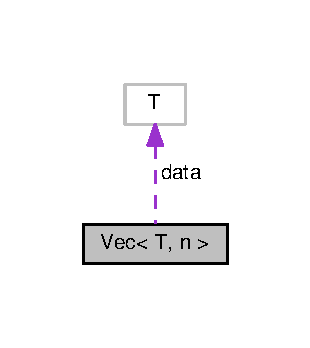
\includegraphics[width=149pt]{structVec__coll__graph}
\end{center}
\end{figure}
\subsection*{Public Member Functions}
\begin{DoxyCompactItemize}
\item 
\hypertarget{structVec_ae64e5410222703c0e8d8a5a84880d9bc}{}H\+E\+M\+I\+\_\+\+D\+E\+V\+\_\+\+C\+A\+L\+L\+A\+B\+L\+E\+\_\+\+I\+N\+L\+I\+N\+E\+\_\+\+M\+E\+M\+B\+E\+R \hyperlink{structVec_ae64e5410222703c0e8d8a5a84880d9bc}{Vec} ()=default\label{structVec_ae64e5410222703c0e8d8a5a84880d9bc}

\begin{DoxyCompactList}\small\item\em Default constructor\+: components uninitialized. \end{DoxyCompactList}\item 
H\+E\+M\+I\+\_\+\+D\+E\+V\+\_\+\+C\+A\+L\+L\+A\+B\+L\+E\+\_\+\+I\+N\+L\+I\+N\+E\+\_\+\+M\+E\+M\+B\+E\+R \hyperlink{structVec_a1105b5b0fea459a6c0d990d717c73552}{Vec} (std\+::initializer\+\_\+list$<$ T $>$ l)
\begin{DoxyCompactList}\small\item\em Initilizer list constructor. \end{DoxyCompactList}\item 
H\+E\+M\+I\+\_\+\+D\+E\+V\+\_\+\+C\+A\+L\+L\+A\+B\+L\+E\+\_\+\+I\+N\+L\+I\+N\+E\+\_\+\+M\+E\+M\+B\+E\+R \hyperlink{structVec_a20483ba3740f996dc2ca12d2b43de450}{Vec} (const T $\ast$const p\+\_\+data)
\begin{DoxyCompactList}\small\item\em Pointer constructor\+: components initilized to pointed data. \end{DoxyCompactList}\item 
H\+E\+M\+I\+\_\+\+D\+E\+V\+\_\+\+C\+A\+L\+L\+A\+B\+L\+E\+\_\+\+I\+N\+L\+I\+N\+E\+\_\+\+M\+E\+M\+B\+E\+R \hyperlink{structVec_a2967598d684273ec428643c9846f733d}{Vec} (const T value)
\begin{DoxyCompactList}\small\item\em Scalar constructor\+: components initilized to scalar value. \end{DoxyCompactList}\item 
\hypertarget{structVec_a504a7837751bbf730dfff159708f1bc9}{}{\footnotesize template$<$typename T\+\_\+out $>$ }\\H\+E\+M\+I\+\_\+\+D\+E\+V\+\_\+\+C\+A\+L\+L\+A\+B\+L\+E\+\_\+\+I\+N\+L\+I\+N\+E\+\_\+\+M\+E\+M\+B\+E\+R \hyperlink{structVec_a504a7837751bbf730dfff159708f1bc9}{operator Vec$<$ T\+\_\+out, n $>$} ()\label{structVec_a504a7837751bbf730dfff159708f1bc9}

\begin{DoxyCompactList}\small\item\em Cast operator\+: static\+\_\+cast() components of n-\/dim \hyperlink{structVec}{Vec}. \end{DoxyCompactList}\item 
H\+E\+M\+I\+\_\+\+D\+E\+V\+\_\+\+C\+A\+L\+L\+A\+B\+L\+E\+\_\+\+I\+N\+L\+I\+N\+E\+\_\+\+M\+E\+M\+B\+E\+R T \& \hyperlink{structVec_af6ec4db0da7c2dbef9a6ce9d0deb6a17}{operator\mbox{[}$\,$\mbox{]}} (const size\+\_\+t index)
\begin{DoxyCompactList}\small\item\em Subscript operator\+: access vector components with bracket notation. \end{DoxyCompactList}\item 
H\+E\+M\+I\+\_\+\+D\+E\+V\+\_\+\+C\+A\+L\+L\+A\+B\+L\+E\+\_\+\+I\+N\+L\+I\+N\+E\+\_\+\+M\+E\+M\+B\+E\+R const T \& \hyperlink{structVec_ac55be8681c862fa0a6d8c75be29d0dc2}{operator\mbox{[}$\,$\mbox{]}} (const size\+\_\+t index) const 
\begin{DoxyCompactList}\small\item\em Const subscript operator\+: access vector components with bracket notation. \end{DoxyCompactList}\end{DoxyCompactItemize}
\subsection*{Public Attributes}
\begin{DoxyCompactItemize}
\item 
\hypertarget{structVec_a76e66063a9a758a351bfd29d104df470}{}T \hyperlink{structVec_a76e66063a9a758a351bfd29d104df470}{data} \mbox{[}n\mbox{]}\label{structVec_a76e66063a9a758a351bfd29d104df470}

\begin{DoxyCompactList}\small\item\em Component storage. \end{DoxyCompactList}\end{DoxyCompactItemize}


\subsection{Detailed Description}
\subsubsection*{template$<$typename T, int n$>$struct Vec$<$ T, n $>$}

Generic n-\/dim \hyperlink{structVec}{Vec} implementation. 

Specialization for 3-\/dim \hyperlink{structVec}{Vec}.

Specialization for 2-\/dim \hyperlink{structVec}{Vec}.


\begin{DoxyTemplParams}{Template Parameters}
{\em T} & component type \\
\hline
{\em n} & dimension \\
\hline
\end{DoxyTemplParams}


\subsection{Constructor \& Destructor Documentation}
\hypertarget{structVec_a1105b5b0fea459a6c0d990d717c73552}{}\index{Vec@{Vec}!Vec@{Vec}}
\index{Vec@{Vec}!Vec@{Vec}}
\subsubsection[{Vec}]{\setlength{\rightskip}{0pt plus 5cm}template$<$typename T, int n$>$ H\+E\+M\+I\+\_\+\+D\+E\+V\+\_\+\+C\+A\+L\+L\+A\+B\+L\+E\+\_\+\+I\+N\+L\+I\+N\+E\+\_\+\+M\+E\+M\+B\+E\+R {\bf Vec}$<$ T, n $>$\+::{\bf Vec} (
\begin{DoxyParamCaption}
\item[{std\+::initializer\+\_\+list$<$ T $>$}]{l}
\end{DoxyParamCaption}
)\hspace{0.3cm}{\ttfamily [inline]}, {\ttfamily [explicit]}}\label{structVec_a1105b5b0fea459a6c0d990d717c73552}


Initilizer list constructor. 


\begin{DoxyParams}[1]{Parameters}
\mbox{\tt in}  & {\em l} & initilizer list \\
\hline
\end{DoxyParams}
\hypertarget{structVec_a20483ba3740f996dc2ca12d2b43de450}{}\index{Vec@{Vec}!Vec@{Vec}}
\index{Vec@{Vec}!Vec@{Vec}}
\subsubsection[{Vec}]{\setlength{\rightskip}{0pt plus 5cm}template$<$typename T, int n$>$ H\+E\+M\+I\+\_\+\+D\+E\+V\+\_\+\+C\+A\+L\+L\+A\+B\+L\+E\+\_\+\+I\+N\+L\+I\+N\+E\+\_\+\+M\+E\+M\+B\+E\+R {\bf Vec}$<$ T, n $>$\+::{\bf Vec} (
\begin{DoxyParamCaption}
\item[{const T $\ast$const}]{p\+\_\+data}
\end{DoxyParamCaption}
)\hspace{0.3cm}{\ttfamily [inline]}, {\ttfamily [explicit]}}\label{structVec_a20483ba3740f996dc2ca12d2b43de450}


Pointer constructor\+: components initilized to pointed data. 


\begin{DoxyParams}[1]{Parameters}
\mbox{\tt in}  & {\em p\+\_\+data} & pointer to data \\
\hline
\end{DoxyParams}
\hypertarget{structVec_a2967598d684273ec428643c9846f733d}{}\index{Vec@{Vec}!Vec@{Vec}}
\index{Vec@{Vec}!Vec@{Vec}}
\subsubsection[{Vec}]{\setlength{\rightskip}{0pt plus 5cm}template$<$typename T, int n$>$ H\+E\+M\+I\+\_\+\+D\+E\+V\+\_\+\+C\+A\+L\+L\+A\+B\+L\+E\+\_\+\+I\+N\+L\+I\+N\+E\+\_\+\+M\+E\+M\+B\+E\+R {\bf Vec}$<$ T, n $>$\+::{\bf Vec} (
\begin{DoxyParamCaption}
\item[{const T}]{value}
\end{DoxyParamCaption}
)\hspace{0.3cm}{\ttfamily [inline]}, {\ttfamily [explicit]}}\label{structVec_a2967598d684273ec428643c9846f733d}


Scalar constructor\+: components initilized to scalar value. 


\begin{DoxyParams}[1]{Parameters}
\mbox{\tt in}  & {\em value} & scalar component value \\
\hline
\end{DoxyParams}


\subsection{Member Function Documentation}
\hypertarget{structVec_af6ec4db0da7c2dbef9a6ce9d0deb6a17}{}\index{Vec@{Vec}!operator\mbox{[}$\,$\mbox{]}@{operator[]}}
\index{operator\mbox{[}$\,$\mbox{]}@{operator[]}!Vec@{Vec}}
\subsubsection[{operator[]}]{\setlength{\rightskip}{0pt plus 5cm}template$<$typename T, int n$>$ H\+E\+M\+I\+\_\+\+D\+E\+V\+\_\+\+C\+A\+L\+L\+A\+B\+L\+E\+\_\+\+I\+N\+L\+I\+N\+E\+\_\+\+M\+E\+M\+B\+E\+R T\& {\bf Vec}$<$ T, n $>$\+::operator\mbox{[}$\,$\mbox{]} (
\begin{DoxyParamCaption}
\item[{const size\+\_\+t}]{index}
\end{DoxyParamCaption}
)\hspace{0.3cm}{\ttfamily [inline]}}\label{structVec_af6ec4db0da7c2dbef9a6ce9d0deb6a17}


Subscript operator\+: access vector components with bracket notation. 


\begin{DoxyParams}[1]{Parameters}
\mbox{\tt in}  & {\em index} & of element \\
\hline
\end{DoxyParams}
\begin{DoxyReturn}{Returns}
index\textquotesingle{}th element of \hyperlink{structVec}{Vec} 
\end{DoxyReturn}
\hypertarget{structVec_ac55be8681c862fa0a6d8c75be29d0dc2}{}\index{Vec@{Vec}!operator\mbox{[}$\,$\mbox{]}@{operator[]}}
\index{operator\mbox{[}$\,$\mbox{]}@{operator[]}!Vec@{Vec}}
\subsubsection[{operator[]}]{\setlength{\rightskip}{0pt plus 5cm}template$<$typename T, int n$>$ H\+E\+M\+I\+\_\+\+D\+E\+V\+\_\+\+C\+A\+L\+L\+A\+B\+L\+E\+\_\+\+I\+N\+L\+I\+N\+E\+\_\+\+M\+E\+M\+B\+E\+R const T\& {\bf Vec}$<$ T, n $>$\+::operator\mbox{[}$\,$\mbox{]} (
\begin{DoxyParamCaption}
\item[{const size\+\_\+t}]{index}
\end{DoxyParamCaption}
) const\hspace{0.3cm}{\ttfamily [inline]}}\label{structVec_ac55be8681c862fa0a6d8c75be29d0dc2}


Const subscript operator\+: access vector components with bracket notation. 


\begin{DoxyParams}[1]{Parameters}
\mbox{\tt in}  & {\em index} & of element \\
\hline
\end{DoxyParams}
\begin{DoxyReturn}{Returns}
index\textquotesingle{}th element of \hyperlink{structVec}{Vec} 
\end{DoxyReturn}


The documentation for this struct was generated from the following file\+:\begin{DoxyCompactItemize}
\item 
/home/atj/\+Dropbox/\+S\+P\+H\+P\+C/\+Simulation\+\_\+\+C\+C/src/vec.\+h\end{DoxyCompactItemize}

\hypertarget{structVec_3_01T_00_012_01_4}{}\section{Vec$<$ T, 2 $>$ Struct Template Reference}
\label{structVec_3_01T_00_012_01_4}\index{Vec$<$ T, 2 $>$@{Vec$<$ T, 2 $>$}}


Collaboration diagram for Vec$<$ T, 2 $>$\+:\nopagebreak
\begin{figure}[H]
\begin{center}
\leavevmode
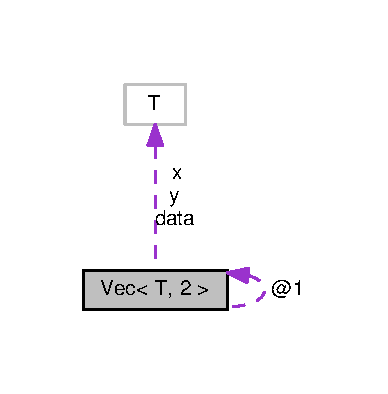
\includegraphics[width=186pt]{structVec_3_01T_00_012_01_4__coll__graph}
\end{center}
\end{figure}
\subsection*{Public Member Functions}
\begin{DoxyCompactItemize}
\item 
\hypertarget{structVec_3_01T_00_012_01_4_ab58ad2db4af2f4ee5ba01094d79b6c62}{}H\+E\+M\+I\+\_\+\+D\+E\+V\+\_\+\+C\+A\+L\+L\+A\+B\+L\+E\+\_\+\+I\+N\+L\+I\+N\+E\+\_\+\+M\+E\+M\+B\+E\+R \hyperlink{structVec_3_01T_00_012_01_4_ab58ad2db4af2f4ee5ba01094d79b6c62}{Vec} ()=default\label{structVec_3_01T_00_012_01_4_ab58ad2db4af2f4ee5ba01094d79b6c62}

\begin{DoxyCompactList}\small\item\em Default constructor\+: components uninitialized. \end{DoxyCompactList}\item 
H\+E\+M\+I\+\_\+\+D\+E\+V\+\_\+\+C\+A\+L\+L\+A\+B\+L\+E\+\_\+\+I\+N\+L\+I\+N\+E\+\_\+\+M\+E\+M\+B\+E\+R \hyperlink{structVec_3_01T_00_012_01_4_ad8e0567970b5b4f69803936d91abc4fe}{Vec} (const T x\+\_\+, const T y\+\_\+)
\begin{DoxyCompactList}\small\item\em Constructor\+: components initilized. \end{DoxyCompactList}\item 
H\+E\+M\+I\+\_\+\+D\+E\+V\+\_\+\+C\+A\+L\+L\+A\+B\+L\+E\+\_\+\+I\+N\+L\+I\+N\+E\+\_\+\+M\+E\+M\+B\+E\+R constexpr \hyperlink{structVec_3_01T_00_012_01_4_a7bd8c58dab2f762360a6061ea4dc6d5f}{Vec} (const T value)
\begin{DoxyCompactList}\small\item\em Constructor\+: components initilized to value. \end{DoxyCompactList}\item 
H\+E\+M\+I\+\_\+\+D\+E\+V\+\_\+\+C\+A\+L\+L\+A\+B\+L\+E\+\_\+\+I\+N\+L\+I\+N\+E\+\_\+\+M\+E\+M\+B\+E\+R constexpr \hyperlink{structVec_3_01T_00_012_01_4_a5091db99b110a4339666121d2714a637}{Vec} (T $\ast$data\+\_\+)
\begin{DoxyCompactList}\small\item\em Pointer constructor\+: components initilized to pointed data. \end{DoxyCompactList}\item 
H\+E\+M\+I\+\_\+\+D\+E\+V\+\_\+\+C\+A\+L\+L\+A\+B\+L\+E\+\_\+\+I\+N\+L\+I\+N\+E\+\_\+\+M\+E\+M\+B\+E\+R constexpr \hyperlink{structVec_3_01T_00_012_01_4_a4e8bf5c102a63649a9728423520b2e7b}{Vec} (const \hyperlink{structVec}{Vec}$<$ T, 3 $>$ \&vec)
\begin{DoxyCompactList}\small\item\em Construct Vec2 from Vec3 by truncating z. \end{DoxyCompactList}\item 
\hypertarget{structVec_3_01T_00_012_01_4_a30c6261be3fb6aa343df595bd94cb8a9}{}{\footnotesize template$<$typename T\+\_\+out $>$ }\\H\+E\+M\+I\+\_\+\+D\+E\+V\+\_\+\+C\+A\+L\+L\+A\+B\+L\+E\+\_\+\+I\+N\+L\+I\+N\+E\+\_\+\+M\+E\+M\+B\+E\+R \hyperlink{structVec_3_01T_00_012_01_4_a30c6261be3fb6aa343df595bd94cb8a9}{operator Vec$<$ T\+\_\+out, 2 $>$} () const \label{structVec_3_01T_00_012_01_4_a30c6261be3fb6aa343df595bd94cb8a9}

\begin{DoxyCompactList}\small\item\em Cast operator\+: static\+\_\+cast() data of Vec2. \end{DoxyCompactList}\item 
H\+E\+M\+I\+\_\+\+D\+E\+V\+\_\+\+C\+A\+L\+L\+A\+B\+L\+E\+\_\+\+I\+N\+L\+I\+N\+E\+\_\+\+M\+E\+M\+B\+E\+R T \& \hyperlink{structVec_3_01T_00_012_01_4_acd3229385a54855ca6b6ba1b94ba7bd0}{operator\mbox{[}$\,$\mbox{]}} (const size\+\_\+t index)
\begin{DoxyCompactList}\small\item\em Subscript operator\+: access vector components with bracket notation. \end{DoxyCompactList}\item 
H\+E\+M\+I\+\_\+\+D\+E\+V\+\_\+\+C\+A\+L\+L\+A\+B\+L\+E\+\_\+\+I\+N\+L\+I\+N\+E\+\_\+\+M\+E\+M\+B\+E\+R const T \& \hyperlink{structVec_3_01T_00_012_01_4_af11a9d4e21ebcdbae1c35b754a22e69b}{operator\mbox{[}$\,$\mbox{]}} (const size\+\_\+t index) const 
\begin{DoxyCompactList}\small\item\em Const subscript operator\+: access vector components with bracket notation. \end{DoxyCompactList}\end{DoxyCompactItemize}
\subsection*{Public Attributes}
\begin{DoxyCompactItemize}
\item 
\hypertarget{structVec_3_01T_00_012_01_4_a38844b2b0447015980a24fcb486e8fd3}{}union \hyperlink{structVec}{Vec}$<$ T, 2 $>$\+:: \{ ... \}  \label{structVec_3_01T_00_012_01_4_a38844b2b0447015980a24fcb486e8fd3}

\begin{DoxyCompactList}\small\item\em union component storage \end{DoxyCompactList}\item 
T \hyperlink{structVec_3_01T_00_012_01_4_ae4ac0867198b0697cc3f9972851ecb94}{data} \mbox{[}2\mbox{]}
\item 
\hypertarget{structVec_3_01T_00_012_01_4_ad8657537de988ece0583a6a2177bbf5f}{}T {\bfseries x}\label{structVec_3_01T_00_012_01_4_ad8657537de988ece0583a6a2177bbf5f}

\item 
\hypertarget{structVec_3_01T_00_012_01_4_a6f8cdcdf206f3a77f3c50e90c721fea0}{}T {\bfseries y}\label{structVec_3_01T_00_012_01_4_a6f8cdcdf206f3a77f3c50e90c721fea0}

\end{DoxyCompactItemize}


\subsection{Constructor \& Destructor Documentation}
\hypertarget{structVec_3_01T_00_012_01_4_ad8e0567970b5b4f69803936d91abc4fe}{}\index{Vec$<$ T, 2 $>$@{Vec$<$ T, 2 $>$}!Vec@{Vec}}
\index{Vec@{Vec}!Vec$<$ T, 2 $>$@{Vec$<$ T, 2 $>$}}
\subsubsection[{Vec}]{\setlength{\rightskip}{0pt plus 5cm}template$<$typename T $>$ H\+E\+M\+I\+\_\+\+D\+E\+V\+\_\+\+C\+A\+L\+L\+A\+B\+L\+E\+\_\+\+I\+N\+L\+I\+N\+E\+\_\+\+M\+E\+M\+B\+E\+R {\bf Vec}$<$ T, 2 $>$\+::{\bf Vec} (
\begin{DoxyParamCaption}
\item[{const T}]{x\+\_\+, }
\item[{const T}]{y\+\_\+}
\end{DoxyParamCaption}
)\hspace{0.3cm}{\ttfamily [inline]}, {\ttfamily [explicit]}}\label{structVec_3_01T_00_012_01_4_ad8e0567970b5b4f69803936d91abc4fe}


Constructor\+: components initilized. 


\begin{DoxyParams}[1]{Parameters}
\mbox{\tt in}  & {\em x\+\_\+} & x component \\
\hline
\mbox{\tt in}  & {\em y\+\_\+} & y component \\
\hline
\end{DoxyParams}
\hypertarget{structVec_3_01T_00_012_01_4_a7bd8c58dab2f762360a6061ea4dc6d5f}{}\index{Vec$<$ T, 2 $>$@{Vec$<$ T, 2 $>$}!Vec@{Vec}}
\index{Vec@{Vec}!Vec$<$ T, 2 $>$@{Vec$<$ T, 2 $>$}}
\subsubsection[{Vec}]{\setlength{\rightskip}{0pt plus 5cm}template$<$typename T $>$ H\+E\+M\+I\+\_\+\+D\+E\+V\+\_\+\+C\+A\+L\+L\+A\+B\+L\+E\+\_\+\+I\+N\+L\+I\+N\+E\+\_\+\+M\+E\+M\+B\+E\+R constexpr {\bf Vec}$<$ T, 2 $>$\+::{\bf Vec} (
\begin{DoxyParamCaption}
\item[{const T}]{value}
\end{DoxyParamCaption}
)\hspace{0.3cm}{\ttfamily [inline]}, {\ttfamily [explicit]}}\label{structVec_3_01T_00_012_01_4_a7bd8c58dab2f762360a6061ea4dc6d5f}


Constructor\+: components initilized to value. 


\begin{DoxyParams}[1]{Parameters}
\mbox{\tt in}  & {\em value} & x, y component \\
\hline
\end{DoxyParams}
\hypertarget{structVec_3_01T_00_012_01_4_a5091db99b110a4339666121d2714a637}{}\index{Vec$<$ T, 2 $>$@{Vec$<$ T, 2 $>$}!Vec@{Vec}}
\index{Vec@{Vec}!Vec$<$ T, 2 $>$@{Vec$<$ T, 2 $>$}}
\subsubsection[{Vec}]{\setlength{\rightskip}{0pt plus 5cm}template$<$typename T $>$ H\+E\+M\+I\+\_\+\+D\+E\+V\+\_\+\+C\+A\+L\+L\+A\+B\+L\+E\+\_\+\+I\+N\+L\+I\+N\+E\+\_\+\+M\+E\+M\+B\+E\+R constexpr {\bf Vec}$<$ T, 2 $>$\+::{\bf Vec} (
\begin{DoxyParamCaption}
\item[{T $\ast$}]{data\+\_\+}
\end{DoxyParamCaption}
)\hspace{0.3cm}{\ttfamily [inline]}, {\ttfamily [explicit]}}\label{structVec_3_01T_00_012_01_4_a5091db99b110a4339666121d2714a637}


Pointer constructor\+: components initilized to pointed data. 


\begin{DoxyParams}[1]{Parameters}
\mbox{\tt in}  & {\em p\+\_\+data} & pointer to data \\
\hline
\end{DoxyParams}
\hypertarget{structVec_3_01T_00_012_01_4_a4e8bf5c102a63649a9728423520b2e7b}{}\index{Vec$<$ T, 2 $>$@{Vec$<$ T, 2 $>$}!Vec@{Vec}}
\index{Vec@{Vec}!Vec$<$ T, 2 $>$@{Vec$<$ T, 2 $>$}}
\subsubsection[{Vec}]{\setlength{\rightskip}{0pt plus 5cm}template$<$typename T $>$ H\+E\+M\+I\+\_\+\+D\+E\+V\+\_\+\+C\+A\+L\+L\+A\+B\+L\+E\+\_\+\+I\+N\+L\+I\+N\+E\+\_\+\+M\+E\+M\+B\+E\+R constexpr {\bf Vec}$<$ T, 2 $>$\+::{\bf Vec} (
\begin{DoxyParamCaption}
\item[{const {\bf Vec}$<$ T, 3 $>$ \&}]{vec}
\end{DoxyParamCaption}
)\hspace{0.3cm}{\ttfamily [inline]}, {\ttfamily [explicit]}}\label{structVec_3_01T_00_012_01_4_a4e8bf5c102a63649a9728423520b2e7b}


Construct Vec2 from Vec3 by truncating z. 


\begin{DoxyParams}[1]{Parameters}
\mbox{\tt in}  & {\em vec} & input Vec3 \\
\hline
\end{DoxyParams}


\subsection{Member Function Documentation}
\hypertarget{structVec_3_01T_00_012_01_4_acd3229385a54855ca6b6ba1b94ba7bd0}{}\index{Vec$<$ T, 2 $>$@{Vec$<$ T, 2 $>$}!operator\mbox{[}$\,$\mbox{]}@{operator[]}}
\index{operator\mbox{[}$\,$\mbox{]}@{operator[]}!Vec$<$ T, 2 $>$@{Vec$<$ T, 2 $>$}}
\subsubsection[{operator[]}]{\setlength{\rightskip}{0pt plus 5cm}template$<$typename T $>$ H\+E\+M\+I\+\_\+\+D\+E\+V\+\_\+\+C\+A\+L\+L\+A\+B\+L\+E\+\_\+\+I\+N\+L\+I\+N\+E\+\_\+\+M\+E\+M\+B\+E\+R T\& {\bf Vec}$<$ T, 2 $>$\+::operator\mbox{[}$\,$\mbox{]} (
\begin{DoxyParamCaption}
\item[{const size\+\_\+t}]{index}
\end{DoxyParamCaption}
)\hspace{0.3cm}{\ttfamily [inline]}}\label{structVec_3_01T_00_012_01_4_acd3229385a54855ca6b6ba1b94ba7bd0}


Subscript operator\+: access vector components with bracket notation. 


\begin{DoxyParams}[1]{Parameters}
\mbox{\tt in}  & {\em index} & of element \\
\hline
\end{DoxyParams}
\begin{DoxyReturn}{Returns}
index\textquotesingle{}th element of \hyperlink{structVec}{Vec} 
\end{DoxyReturn}
\hypertarget{structVec_3_01T_00_012_01_4_af11a9d4e21ebcdbae1c35b754a22e69b}{}\index{Vec$<$ T, 2 $>$@{Vec$<$ T, 2 $>$}!operator\mbox{[}$\,$\mbox{]}@{operator[]}}
\index{operator\mbox{[}$\,$\mbox{]}@{operator[]}!Vec$<$ T, 2 $>$@{Vec$<$ T, 2 $>$}}
\subsubsection[{operator[]}]{\setlength{\rightskip}{0pt plus 5cm}template$<$typename T $>$ H\+E\+M\+I\+\_\+\+D\+E\+V\+\_\+\+C\+A\+L\+L\+A\+B\+L\+E\+\_\+\+I\+N\+L\+I\+N\+E\+\_\+\+M\+E\+M\+B\+E\+R const T\& {\bf Vec}$<$ T, 2 $>$\+::operator\mbox{[}$\,$\mbox{]} (
\begin{DoxyParamCaption}
\item[{const size\+\_\+t}]{index}
\end{DoxyParamCaption}
) const\hspace{0.3cm}{\ttfamily [inline]}}\label{structVec_3_01T_00_012_01_4_af11a9d4e21ebcdbae1c35b754a22e69b}


Const subscript operator\+: access vector components with bracket notation. 


\begin{DoxyParams}[1]{Parameters}
\mbox{\tt in}  & {\em index} & of element \\
\hline
\end{DoxyParams}
\begin{DoxyReturn}{Returns}
index\textquotesingle{}th element of \hyperlink{structVec}{Vec} 
\end{DoxyReturn}


\subsection{Member Data Documentation}
\hypertarget{structVec_3_01T_00_012_01_4_ae4ac0867198b0697cc3f9972851ecb94}{}\index{Vec$<$ T, 2 $>$@{Vec$<$ T, 2 $>$}!data@{data}}
\index{data@{data}!Vec$<$ T, 2 $>$@{Vec$<$ T, 2 $>$}}
\subsubsection[{data}]{\setlength{\rightskip}{0pt plus 5cm}template$<$typename T $>$ T {\bf Vec}$<$ T, 2 $>$\+::data\mbox{[}2\mbox{]}}\label{structVec_3_01T_00_012_01_4_ae4ac0867198b0697cc3f9972851ecb94}
component array 

The documentation for this struct was generated from the following file\+:\begin{DoxyCompactItemize}
\item 
/home/atj/\+Dropbox/\+S\+P\+H\+P\+C/\+Simulation\+\_\+\+C\+C/src/vec.\+h\end{DoxyCompactItemize}

\hypertarget{structVec_3_01T_00_013_01_4}{}\section{Vec$<$ T, 3 $>$ Struct Template Reference}
\label{structVec_3_01T_00_013_01_4}\index{Vec$<$ T, 3 $>$@{Vec$<$ T, 3 $>$}}


Collaboration diagram for Vec$<$ T, 3 $>$\+:\nopagebreak
\begin{figure}[H]
\begin{center}
\leavevmode
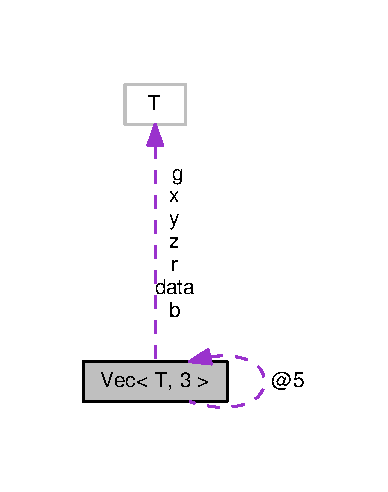
\includegraphics[width=186pt]{structVec_3_01T_00_013_01_4__coll__graph}
\end{center}
\end{figure}
\subsection*{Public Member Functions}
\begin{DoxyCompactItemize}
\item 
\hypertarget{structVec_3_01T_00_013_01_4_a0067c7aff3900cdb7180a2a43081cde9}{}\hyperlink{structVec_3_01T_00_013_01_4_a0067c7aff3900cdb7180a2a43081cde9}{Vec} ()=default\label{structVec_3_01T_00_013_01_4_a0067c7aff3900cdb7180a2a43081cde9}

\begin{DoxyCompactList}\small\item\em Default constructor\+: components uninitialized. \end{DoxyCompactList}\item 
\hyperlink{structVec_3_01T_00_013_01_4_a5b7405b3d5de4da6f3ae64a34ded20f2}{Vec} (const T x\+\_\+, const T y\+\_\+, const T z\+\_\+)
\begin{DoxyCompactList}\small\item\em Constructor\+: components initilized. \end{DoxyCompactList}\item 
constexpr \hyperlink{structVec_3_01T_00_013_01_4_ac72d7e468df1e33d4ab3fead9220b604}{Vec} (const T value)
\begin{DoxyCompactList}\small\item\em Constructor\+: components initilized to value. \end{DoxyCompactList}\item 
constexpr \hyperlink{structVec_3_01T_00_013_01_4_aca9ea0df8cd8e4301ae0fa7fd7d2f27e}{Vec} (T $\ast$data\+\_\+)
\begin{DoxyCompactList}\small\item\em Pointer constructor\+: components initilized to pointed data. \end{DoxyCompactList}\item 
\hyperlink{structVec_3_01T_00_013_01_4_a0c974365e952d0cd79979c9483ad2ae8}{Vec} (const \hyperlink{structVec}{Vec}$<$ T, 2 $>$ \&vec\+\_\+)
\begin{DoxyCompactList}\small\item\em Construct Vec2 from Vec3 by setting z to 0. \end{DoxyCompactList}\item 
\hyperlink{structVec_3_01T_00_013_01_4_a443a51b3428cb74e590654c4bd174a85}{Vec} (const \hyperlink{structVec}{Vec}$<$ T, 2 $>$ \&vec\+\_\+, T z\+\_\+)
\begin{DoxyCompactList}\small\item\em Construct Vec2 from Vec3 by specifying z. \end{DoxyCompactList}\item 
\hypertarget{structVec_3_01T_00_013_01_4_aec0f2f9c0ba16854de1fb1547530daa2}{}{\footnotesize template$<$typename T\+\_\+out $>$ }\\\hyperlink{structVec_3_01T_00_013_01_4_aec0f2f9c0ba16854de1fb1547530daa2}{operator Vec$<$ T\+\_\+out, 3 $>$} () const \label{structVec_3_01T_00_013_01_4_aec0f2f9c0ba16854de1fb1547530daa2}

\begin{DoxyCompactList}\small\item\em Cast operator\+: static\+\_\+cast() data of Vec3. \end{DoxyCompactList}\item 
T \& \hyperlink{structVec_3_01T_00_013_01_4_a5f0a78557890a6d86d0ac2282426217b}{operator\mbox{[}$\,$\mbox{]}} (const size\+\_\+t index)
\begin{DoxyCompactList}\small\item\em Subscript operator\+: access vector components with bracket notation. \end{DoxyCompactList}\item 
const T \& \hyperlink{structVec_3_01T_00_013_01_4_af2d3eabac7af9dfa72a89b3370a24ed2}{operator\mbox{[}$\,$\mbox{]}} (const size\+\_\+t index) const 
\begin{DoxyCompactList}\small\item\em Const subscript operator\+: access vector components with bracket notation. \end{DoxyCompactList}\end{DoxyCompactItemize}
\subsection*{Public Attributes}
\begin{DoxyCompactItemize}
\item 
\hypertarget{structVec_3_01T_00_013_01_4_a090a6e6d6471482a33d4f5b66548c9e5}{}union \hyperlink{structVec}{Vec}$<$ T, 3 $>$\+:: \{ ... \}  \label{structVec_3_01T_00_013_01_4_a090a6e6d6471482a33d4f5b66548c9e5}

\item 
T \hyperlink{structVec_3_01T_00_013_01_4_a07af69736eca9e1115b69d51fac21514}{data} \mbox{[}3\mbox{]}
\item 
\hypertarget{structVec_3_01T_00_013_01_4_ac73cf62d6ee2d6f72a40a6d30677e2c5}{}T {\bfseries x}\label{structVec_3_01T_00_013_01_4_ac73cf62d6ee2d6f72a40a6d30677e2c5}

\item 
\hypertarget{structVec_3_01T_00_013_01_4_a518370197670c87da6f100853dd1ebe7}{}T {\bfseries y}\label{structVec_3_01T_00_013_01_4_a518370197670c87da6f100853dd1ebe7}

\item 
\hypertarget{structVec_3_01T_00_013_01_4_a380f1acf13bb3e1d570bf3396aa32bb0}{}T {\bfseries z}\label{structVec_3_01T_00_013_01_4_a380f1acf13bb3e1d570bf3396aa32bb0}

\item 
\hypertarget{structVec_3_01T_00_013_01_4_acb3dc926a0256dda915039cdb213596e}{}T {\bfseries r}\label{structVec_3_01T_00_013_01_4_acb3dc926a0256dda915039cdb213596e}

\item 
\hypertarget{structVec_3_01T_00_013_01_4_ab6e2b4d396af0d9cc561b3d4f684dd2c}{}T {\bfseries g}\label{structVec_3_01T_00_013_01_4_ab6e2b4d396af0d9cc561b3d4f684dd2c}

\item 
\hypertarget{structVec_3_01T_00_013_01_4_a5828f123a95e1eeef713612137196a42}{}T {\bfseries b}\label{structVec_3_01T_00_013_01_4_a5828f123a95e1eeef713612137196a42}

\end{DoxyCompactItemize}


\subsection{Constructor \& Destructor Documentation}
\hypertarget{structVec_3_01T_00_013_01_4_a5b7405b3d5de4da6f3ae64a34ded20f2}{}\index{Vec$<$ T, 3 $>$@{Vec$<$ T, 3 $>$}!Vec@{Vec}}
\index{Vec@{Vec}!Vec$<$ T, 3 $>$@{Vec$<$ T, 3 $>$}}
\subsubsection[{Vec}]{\setlength{\rightskip}{0pt plus 5cm}template$<$typename T $>$ {\bf Vec}$<$ T, 3 $>$\+::{\bf Vec} (
\begin{DoxyParamCaption}
\item[{const T}]{x\+\_\+, }
\item[{const T}]{y\+\_\+, }
\item[{const T}]{z\+\_\+}
\end{DoxyParamCaption}
)\hspace{0.3cm}{\ttfamily [inline]}, {\ttfamily [explicit]}}\label{structVec_3_01T_00_013_01_4_a5b7405b3d5de4da6f3ae64a34ded20f2}


Constructor\+: components initilized. 


\begin{DoxyParams}[1]{Parameters}
\mbox{\tt in}  & {\em x\+\_\+} & x component \\
\hline
\mbox{\tt in}  & {\em y\+\_\+} & y component \\
\hline
\mbox{\tt in}  & {\em z\+\_\+} & z component \\
\hline
\end{DoxyParams}
\hypertarget{structVec_3_01T_00_013_01_4_ac72d7e468df1e33d4ab3fead9220b604}{}\index{Vec$<$ T, 3 $>$@{Vec$<$ T, 3 $>$}!Vec@{Vec}}
\index{Vec@{Vec}!Vec$<$ T, 3 $>$@{Vec$<$ T, 3 $>$}}
\subsubsection[{Vec}]{\setlength{\rightskip}{0pt plus 5cm}template$<$typename T $>$ constexpr {\bf Vec}$<$ T, 3 $>$\+::{\bf Vec} (
\begin{DoxyParamCaption}
\item[{const T}]{value}
\end{DoxyParamCaption}
)\hspace{0.3cm}{\ttfamily [inline]}, {\ttfamily [explicit]}}\label{structVec_3_01T_00_013_01_4_ac72d7e468df1e33d4ab3fead9220b604}


Constructor\+: components initilized to value. 


\begin{DoxyParams}[1]{Parameters}
\mbox{\tt in}  & {\em value} & x, y, z component \\
\hline
\end{DoxyParams}
\hypertarget{structVec_3_01T_00_013_01_4_aca9ea0df8cd8e4301ae0fa7fd7d2f27e}{}\index{Vec$<$ T, 3 $>$@{Vec$<$ T, 3 $>$}!Vec@{Vec}}
\index{Vec@{Vec}!Vec$<$ T, 3 $>$@{Vec$<$ T, 3 $>$}}
\subsubsection[{Vec}]{\setlength{\rightskip}{0pt plus 5cm}template$<$typename T $>$ constexpr {\bf Vec}$<$ T, 3 $>$\+::{\bf Vec} (
\begin{DoxyParamCaption}
\item[{T $\ast$}]{data\+\_\+}
\end{DoxyParamCaption}
)\hspace{0.3cm}{\ttfamily [inline]}, {\ttfamily [explicit]}}\label{structVec_3_01T_00_013_01_4_aca9ea0df8cd8e4301ae0fa7fd7d2f27e}


Pointer constructor\+: components initilized to pointed data. 


\begin{DoxyParams}[1]{Parameters}
\mbox{\tt in}  & {\em p\+\_\+data} & pointer to data \\
\hline
\end{DoxyParams}
\hypertarget{structVec_3_01T_00_013_01_4_a0c974365e952d0cd79979c9483ad2ae8}{}\index{Vec$<$ T, 3 $>$@{Vec$<$ T, 3 $>$}!Vec@{Vec}}
\index{Vec@{Vec}!Vec$<$ T, 3 $>$@{Vec$<$ T, 3 $>$}}
\subsubsection[{Vec}]{\setlength{\rightskip}{0pt plus 5cm}template$<$typename T $>$ {\bf Vec}$<$ T, 3 $>$\+::{\bf Vec} (
\begin{DoxyParamCaption}
\item[{const {\bf Vec}$<$ T, 2 $>$ \&}]{vec\+\_\+}
\end{DoxyParamCaption}
)\hspace{0.3cm}{\ttfamily [inline]}, {\ttfamily [explicit]}}\label{structVec_3_01T_00_013_01_4_a0c974365e952d0cd79979c9483ad2ae8}


Construct Vec2 from Vec3 by setting z to 0. 


\begin{DoxyParams}[1]{Parameters}
\mbox{\tt in}  & {\em vec} & Vec2 \\
\hline
\end{DoxyParams}
\hypertarget{structVec_3_01T_00_013_01_4_a443a51b3428cb74e590654c4bd174a85}{}\index{Vec$<$ T, 3 $>$@{Vec$<$ T, 3 $>$}!Vec@{Vec}}
\index{Vec@{Vec}!Vec$<$ T, 3 $>$@{Vec$<$ T, 3 $>$}}
\subsubsection[{Vec}]{\setlength{\rightskip}{0pt plus 5cm}template$<$typename T $>$ {\bf Vec}$<$ T, 3 $>$\+::{\bf Vec} (
\begin{DoxyParamCaption}
\item[{const {\bf Vec}$<$ T, 2 $>$ \&}]{vec\+\_\+, }
\item[{T}]{z\+\_\+}
\end{DoxyParamCaption}
)\hspace{0.3cm}{\ttfamily [inline]}, {\ttfamily [explicit]}}\label{structVec_3_01T_00_013_01_4_a443a51b3428cb74e590654c4bd174a85}


Construct Vec2 from Vec3 by specifying z. 


\begin{DoxyParams}[1]{Parameters}
\mbox{\tt in}  & {\em vec} & Vec2 x,y values \\
\hline
\mbox{\tt in}  & {\em z} & z value \\
\hline
\end{DoxyParams}


\subsection{Member Function Documentation}
\hypertarget{structVec_3_01T_00_013_01_4_a5f0a78557890a6d86d0ac2282426217b}{}\index{Vec$<$ T, 3 $>$@{Vec$<$ T, 3 $>$}!operator\mbox{[}$\,$\mbox{]}@{operator[]}}
\index{operator\mbox{[}$\,$\mbox{]}@{operator[]}!Vec$<$ T, 3 $>$@{Vec$<$ T, 3 $>$}}
\subsubsection[{operator[]}]{\setlength{\rightskip}{0pt plus 5cm}template$<$typename T $>$ T\& {\bf Vec}$<$ T, 3 $>$\+::operator\mbox{[}$\,$\mbox{]} (
\begin{DoxyParamCaption}
\item[{const size\+\_\+t}]{index}
\end{DoxyParamCaption}
)\hspace{0.3cm}{\ttfamily [inline]}}\label{structVec_3_01T_00_013_01_4_a5f0a78557890a6d86d0ac2282426217b}


Subscript operator\+: access vector components with bracket notation. 


\begin{DoxyParams}[1]{Parameters}
\mbox{\tt in}  & {\em index} & of element \\
\hline
\end{DoxyParams}
\begin{DoxyReturn}{Returns}
index\textquotesingle{}th element of \hyperlink{structVec}{Vec} 
\end{DoxyReturn}
\hypertarget{structVec_3_01T_00_013_01_4_af2d3eabac7af9dfa72a89b3370a24ed2}{}\index{Vec$<$ T, 3 $>$@{Vec$<$ T, 3 $>$}!operator\mbox{[}$\,$\mbox{]}@{operator[]}}
\index{operator\mbox{[}$\,$\mbox{]}@{operator[]}!Vec$<$ T, 3 $>$@{Vec$<$ T, 3 $>$}}
\subsubsection[{operator[]}]{\setlength{\rightskip}{0pt plus 5cm}template$<$typename T $>$ const T\& {\bf Vec}$<$ T, 3 $>$\+::operator\mbox{[}$\,$\mbox{]} (
\begin{DoxyParamCaption}
\item[{const size\+\_\+t}]{index}
\end{DoxyParamCaption}
) const\hspace{0.3cm}{\ttfamily [inline]}}\label{structVec_3_01T_00_013_01_4_af2d3eabac7af9dfa72a89b3370a24ed2}


Const subscript operator\+: access vector components with bracket notation. 


\begin{DoxyParams}[1]{Parameters}
\mbox{\tt in}  & {\em index} & of element \\
\hline
\end{DoxyParams}
\begin{DoxyReturn}{Returns}
index\textquotesingle{}th element of \hyperlink{structVec}{Vec} 
\end{DoxyReturn}


\subsection{Member Data Documentation}
\hypertarget{structVec_3_01T_00_013_01_4_a07af69736eca9e1115b69d51fac21514}{}\index{Vec$<$ T, 3 $>$@{Vec$<$ T, 3 $>$}!data@{data}}
\index{data@{data}!Vec$<$ T, 3 $>$@{Vec$<$ T, 3 $>$}}
\subsubsection[{data}]{\setlength{\rightskip}{0pt plus 5cm}template$<$typename T $>$ T {\bf Vec}$<$ T, 3 $>$\+::data\mbox{[}3\mbox{]}}\label{structVec_3_01T_00_013_01_4_a07af69736eca9e1115b69d51fac21514}
component array 

The documentation for this struct was generated from the following file\+:\begin{DoxyCompactItemize}
\item 
/home/atj/\+Dropbox/\+S\+P\+H\+P\+C/\+Simulation\+\_\+\+C\+C/src/vec.\+h\end{DoxyCompactItemize}

%--- End generated contents ---

% Index
\backmatter
\newpage
\phantomsection
\clearemptydoublepage
\addcontentsline{toc}{chapter}{Index}
\printindex

\end{document}
